\section{\small Linear Independence}

A set of non-zero vectors $\{\vec{v}_1, \vec{v}_2, \dots, \vec{v}_k \in
	\mathbb{R}^n\}$ are said to be \textbf{linearly dependent} if there exists real
scalars $\alpha_1, \alpha_2, \dots, \alpha_k$ \textit{not all zero} such that:
\[
	\sum_{i=1}^{k} \alpha_i \vec{v}_i = \vec{0}
\]
In this case, we have $\mathcal{N}(V) \neq 0$.
Conversely, $\{\vec{v}_1, \vec{v}_2, \dots, \vec{v}_k \in \mathbb{R}^n\}$ are
\textbf{linearly independent} if the only solution to the equation:
\[
	\sum_{i=1}^{k} \alpha_i \vec{v}_i \leftrightarrow \alpha_1 = \alpha_2 =
	\ldots = \alpha_k =
	0
\]
In this case, we have $\mathcal{N}(V) = 0$.\\

Given $\vec{b} \in \mathbb{R}^m$, $\vec{x} \in \mathbb{R}^m$, and $\mathbf{A}
	\in \mathbb{R}^{n \times m}$, consider the equation $\mathbf{A} \vec{x} = \vec{b}$.

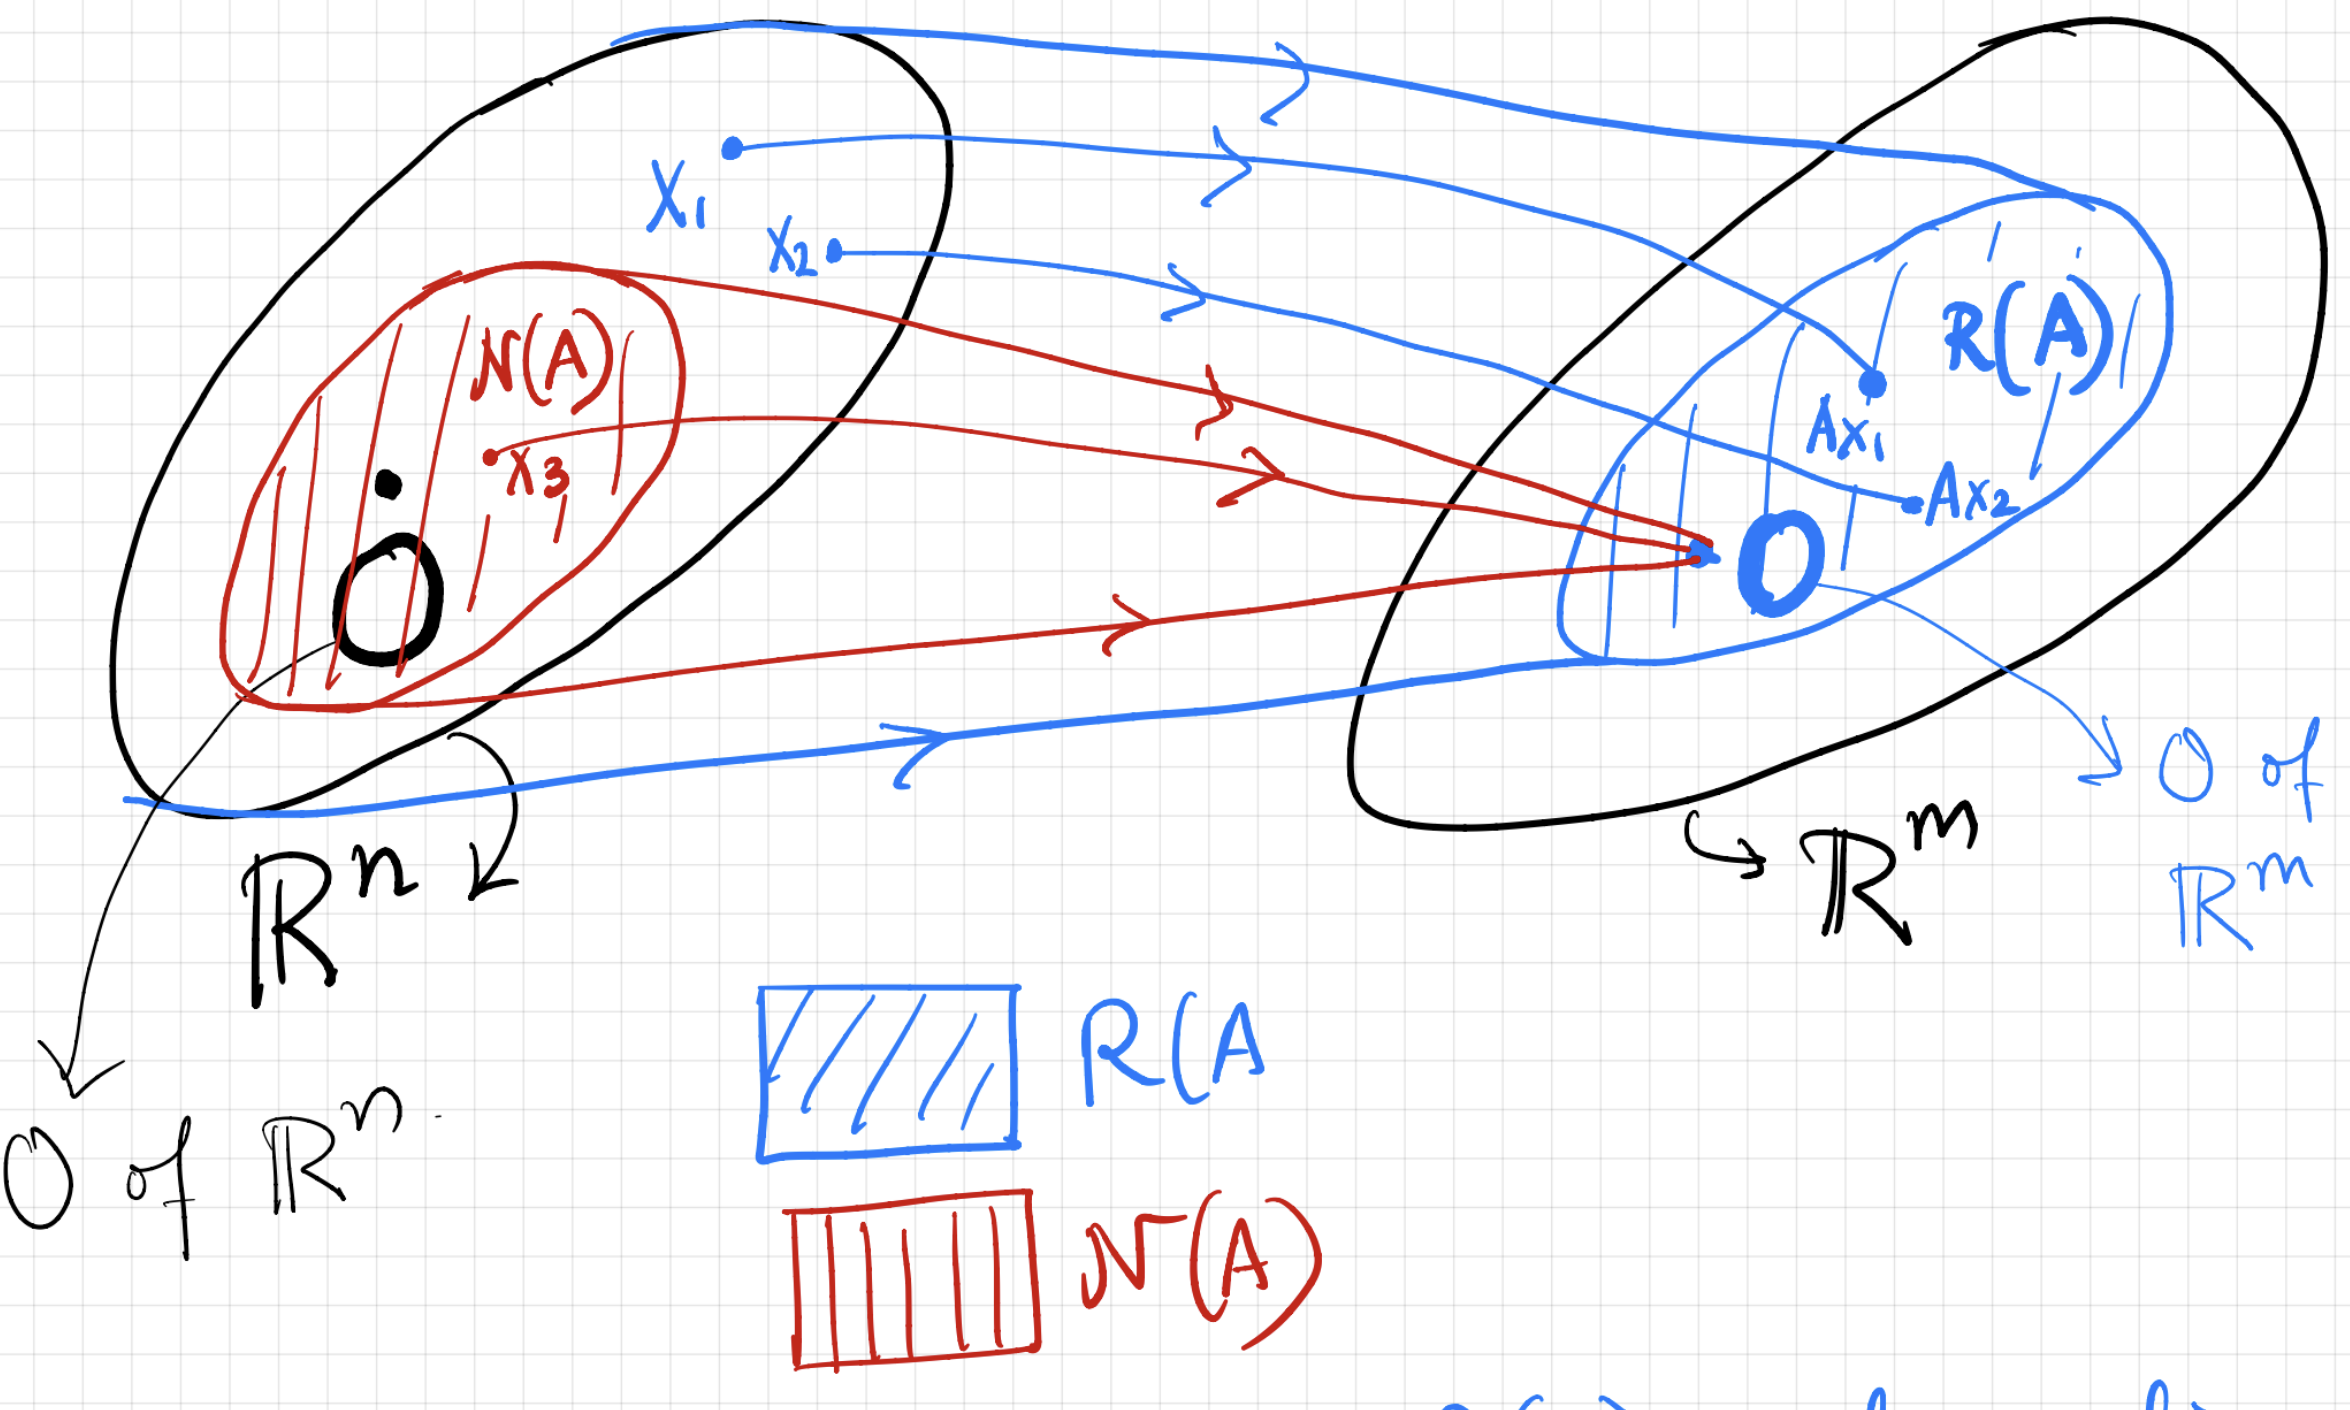
\includegraphics[width=0.2\textwidth]{images/RnRm2.png} \\

The entirety of $\mathbb{R}^n$ is mapped onto $\mathbb{R}^m$ by $\mathbf{A}$
($\vec{x}_k$ maps to $\mathbf{A} \vec{x}_k \in \mathbb{R}^m$). The entirety of
$\mathcal{N}(A) \in \mathbb{R}^n$ is mapped to $\vec{0} \in \mathbb{R}^m$.

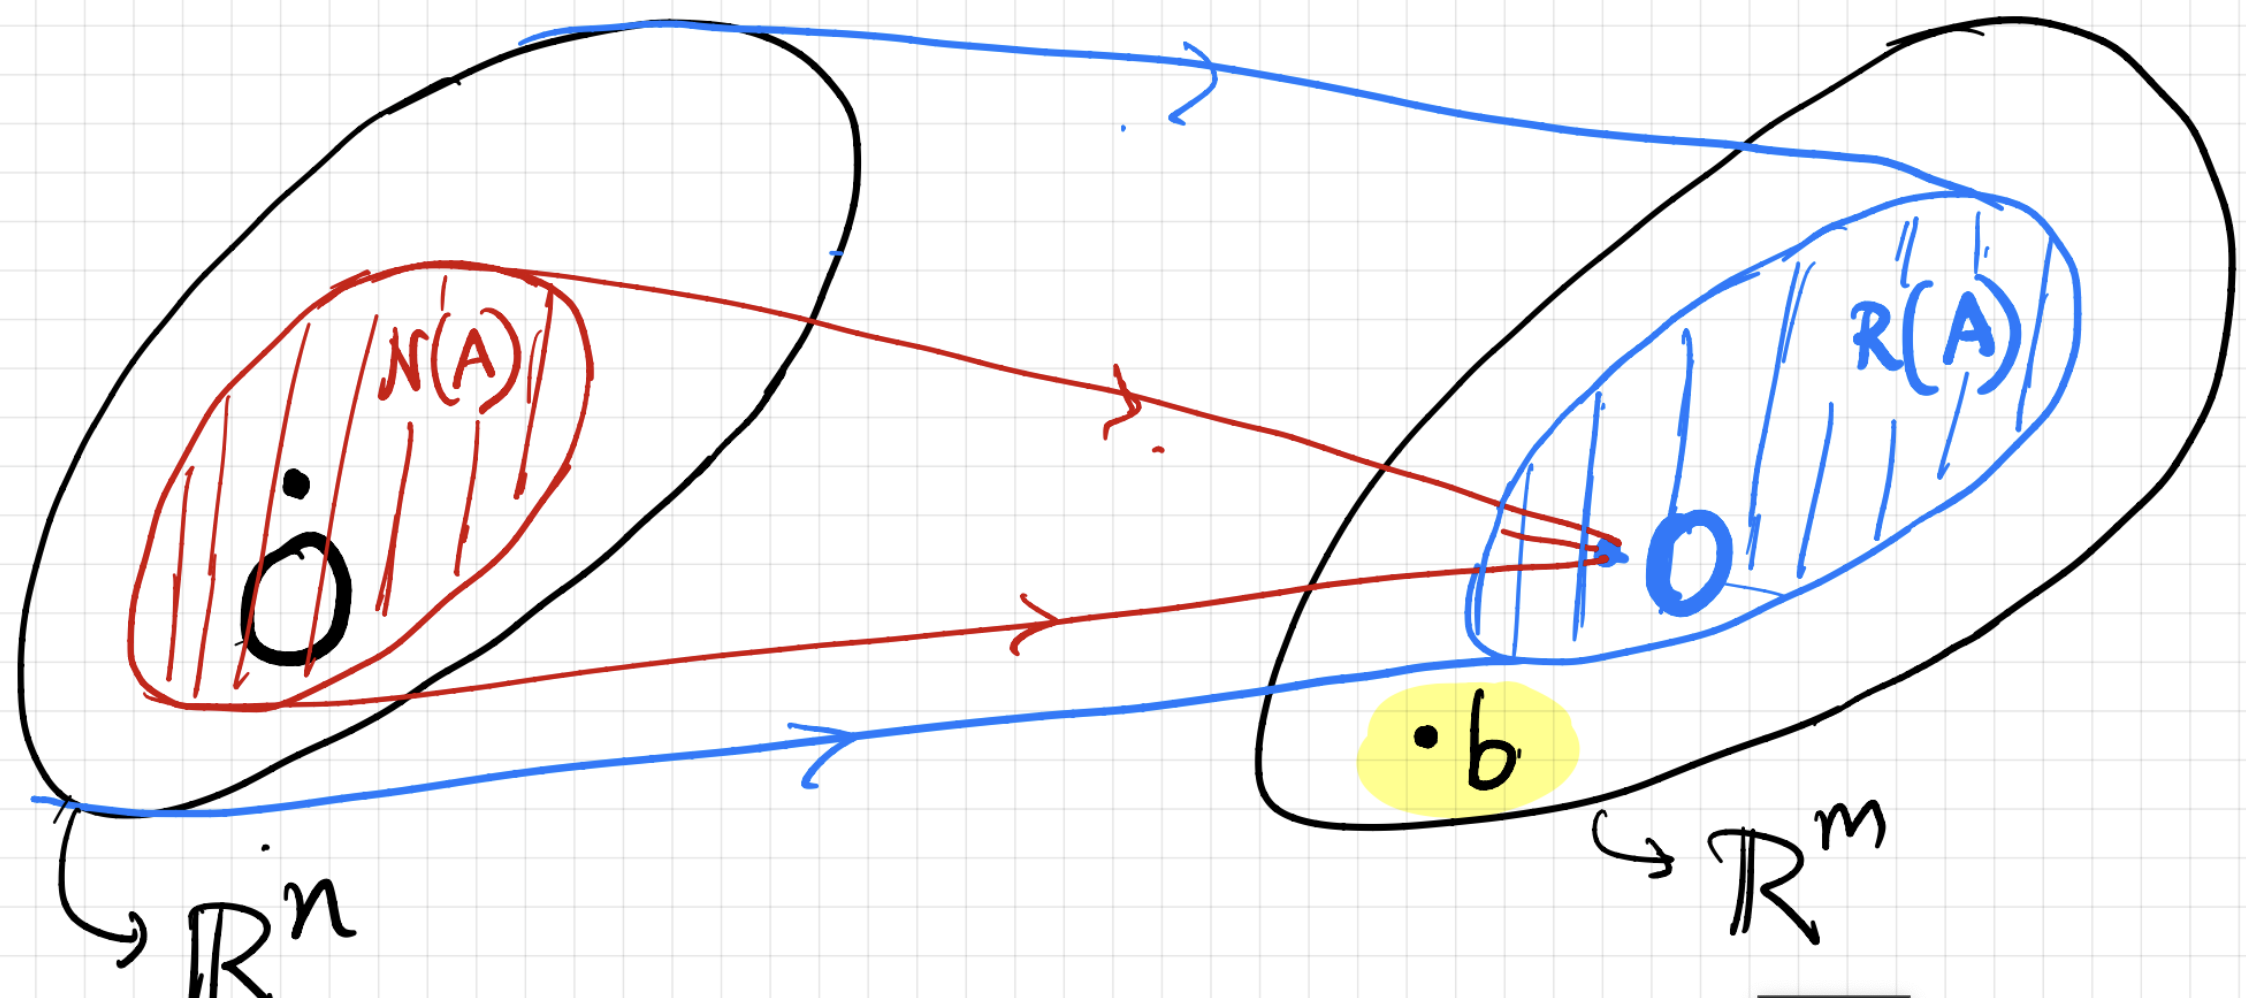
\includegraphics[width=0.2\textwidth]{images/RnRm.png} \\
Now consider $\vec{b}$ which may or may not belong to $\mathcal{R}(A)$. Then we
can use the following to determine the number of solutions:

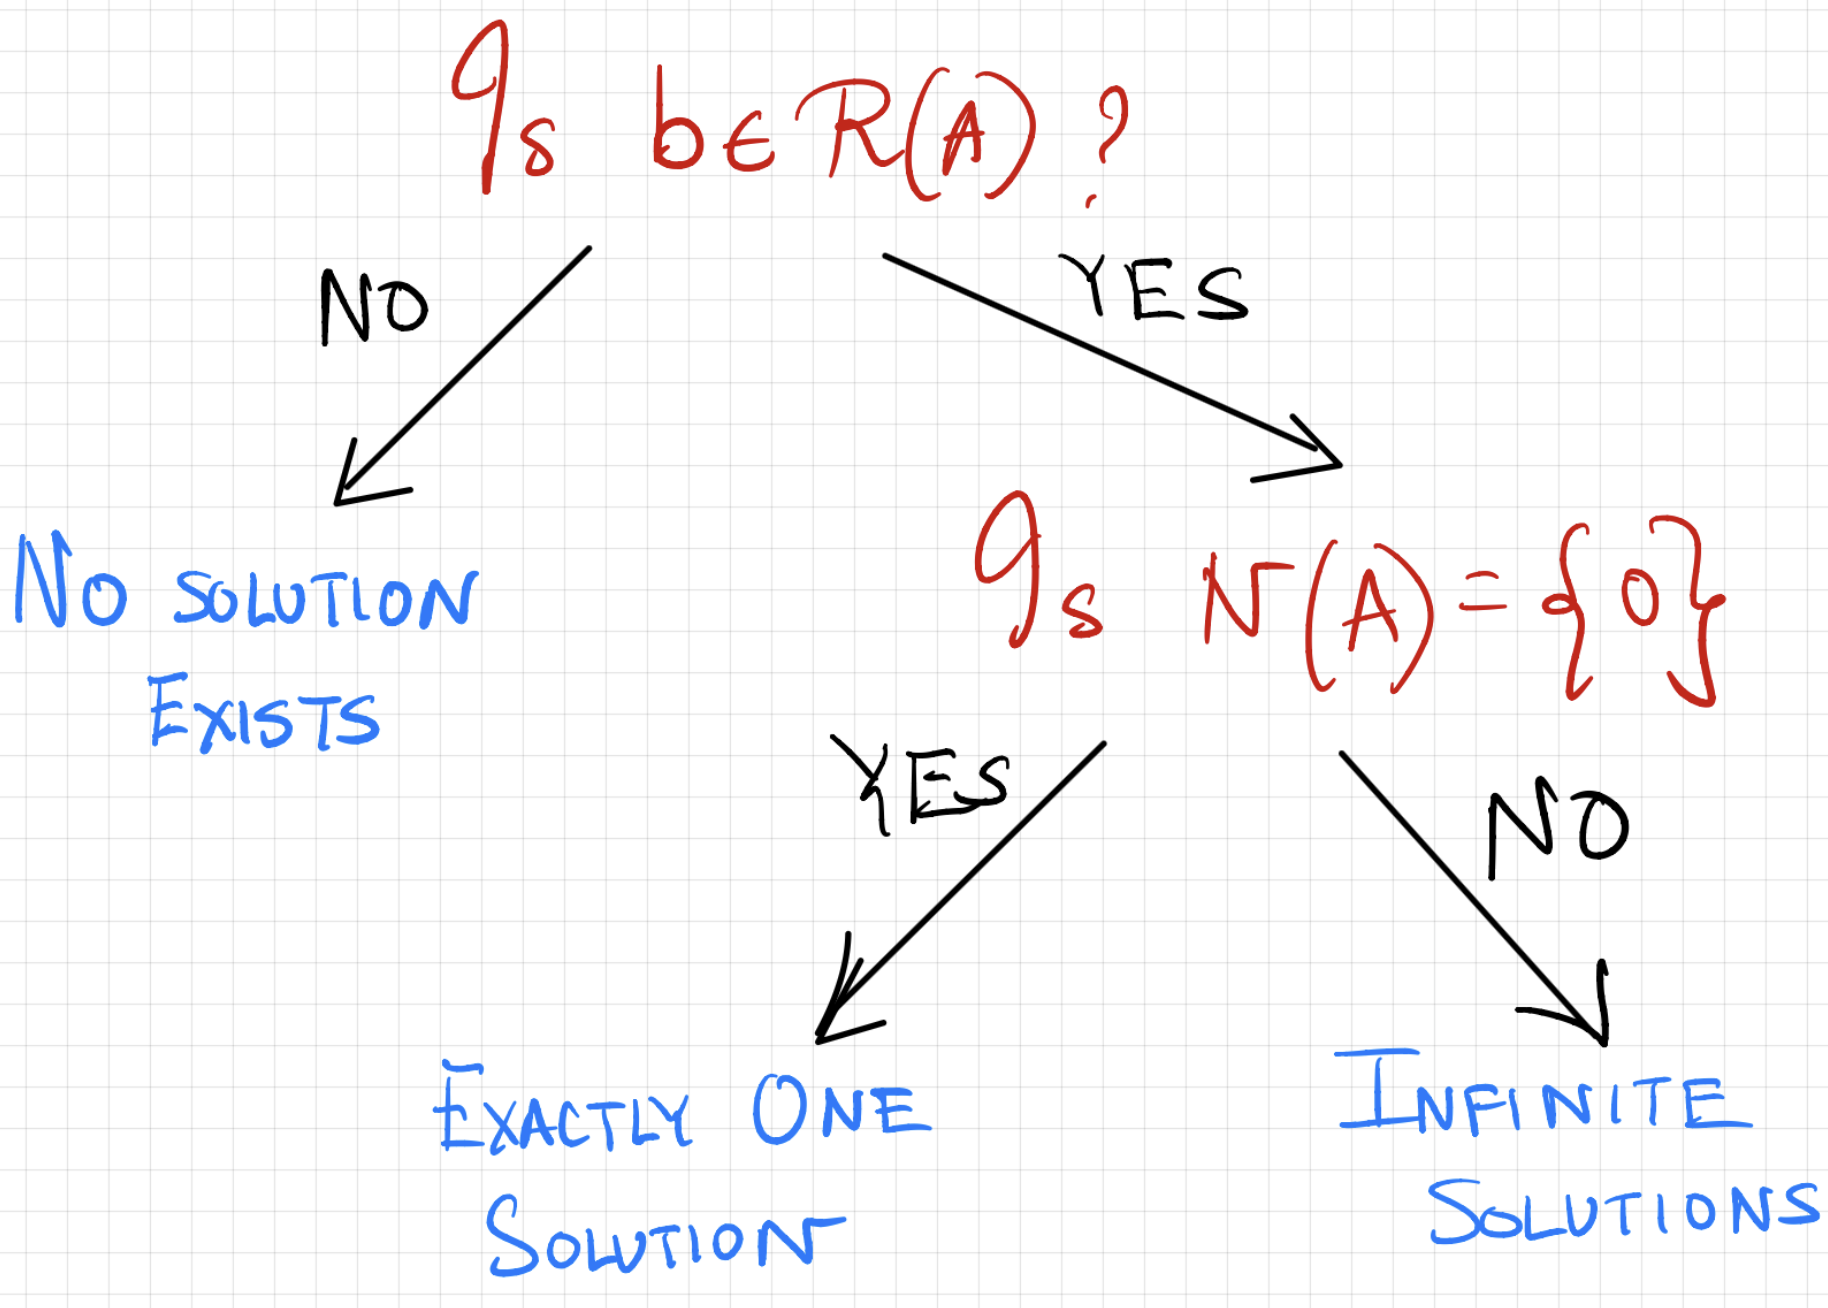
\includegraphics[width=0.2\textwidth]{images/full_picture.png}
